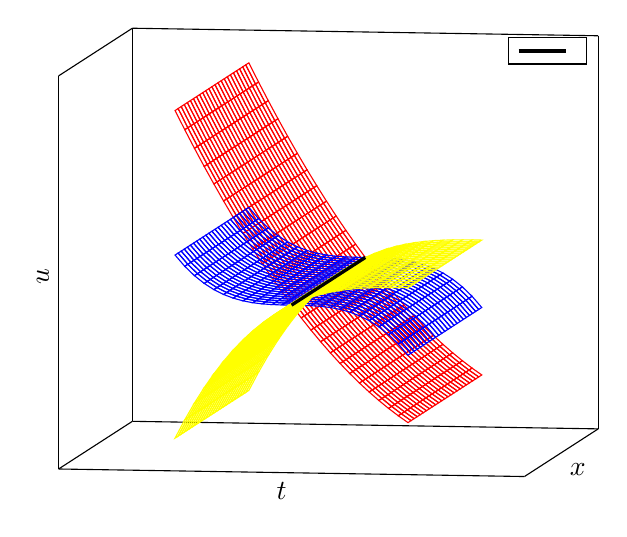
\begin{tikzpicture}
  \begin{axis}[view={99}{7},ticks=none,xlabel=$x$,ylabel=$t$,zlabel=$u$,ymin=-1.,ymax=1.]
    \addplot3[black,very thick,domain=-4:4,samples=60,samples y=0]({x},{0.},{5.});
    \addplot3[mesh,draw=Red,domain=-4:4,y domain=-0.5:0.5] {2.*(y-1.)^2 -2. +5.};
    \addplot3[mesh,draw=Blue,domain=-4:4,y domain=-0.5:0.5] {-5.*y^3+5.};
    \addplot3[mesh,draw=Yellow,domain=-4:4,y domain=-0.5:0.5] {2.*(y-0.5)^3+(2.*(0.5)^3)+5.};
    \addplot3[black,very thick,domain=-4:4,samples=60,samples y=0]({x},{0.},{5.});
    \legend{$\Cscr$}
  \end{axis}
\end{tikzpicture}
%%% Local Variables:
%%% mode: latex
%%% TeX-master: "../../mainManuscript"
%%% End:
